\section{Form of Polyatomic Partition Function}%
\label{sec:polyppf}
With the knowledge of appropriateness to treat particular degrees of freedom
classically, we can approach the topic of polyatomic molecule using an
suitable combination of classical and quantum mechanics. Of course the full
quantum mechanical solution will be strictly more accurate, but not necessarily
usefully more accurate.
\subsection{Approximations}
In order to derive the vibrational and electronic modes, the Born-Oppenheimer
approximation is necessary. In doing so we wish to arrive at a description of
the electronic potential in as a function of a currently unknown number of
variables. To fully describe a polyatomic molecule's position $3n$ coordinates
are needed, where $n$ is the number of atoms in the molecule. 3 coordinates can
describe the center of mass of the particle. 2 $(\theta~\text{and}~\phi)$ or 3
$(\theta,~\phi,~\text{and}~\psi)$ coordinates uniquely specify the rotation of a
rigid linear and non-linear body respectively. This leaves $3n - 5$ or $3n - 6$
degrees of freedom internal to the molecule. Thus, the internal motion of the
molecule occurs in a potential energy landscape of $3n - 5$ or $3n - 6$
dimensions.

Furthermore, in order to deal with vibrational and rotational energy modes
separately, we will make the rigid-rotor harmonic oscillator approximation
again.

\subsection{Translational, Electric, and Nuclear Partition Functions}
The translational partition function is identical to the previous cases except
that we must be careful to define translation as the movement of the center of
mass of the particle. Therefore, the translational partition function is
\begin{equation}
	q_{trans} = {\left(\frac{2\pi mkT}{h^3}\right)}V.
\end{equation}
The electronic partition function is also identical. We set the energy zero
to the energy where all atoms are separated in their ground state, in
other words the ground state is at an energy, $-D_e$. The partition function is
then,
\begin{equation*}
	q_{elect} = \omega_{e1} e^{D_{e}/kT}.
\end{equation*}
We ignore any state other than the ground state for nuclei and set the nuclear
partition function, $q_{nucl} = 1$.

\section{Vibrational Partition Function}%
\label{sec:polyvpf}
Given the previous analysis of the potential energy field of the nuclei of the
molecule, the nuclei vibrate in $(3n - 5)$ or $(3n - 6)$ dimensions. These
relative dimensions will involve combinations of the nuclei's positions such
that in the squaring of terms leave cross terms. An example would be the
combination,
\begin{equation*}
	(x_2 - x_{1})^{2} = x_{2}^2 - 2 x_1 x_2 + x_1^2.
\end{equation*}
The square comes from the assumption that force is roughly linear with small
deviations from the equilibrium positions this is the harmonic oscillator
assumption. Luckily using a method called \textit{normal coordinate analysis}
can determine a set of coordinates $\{Q_{i}\}$ such that each harmonic
oscillator is devoid of cross terms. The Hamiltonian is thus
\begin{align*}
	\H &= K + U\\
	   &= - \sum_{j=1}^{\alpha}{\frac{\hbar^2}{2 \mu_j}
	\frac{\partial^2}{\partial Q_j^2}} +
	\sum_{j=1}^{\alpha}{\frac{k_j}{2}Q_{j^2}} \quad \alpha = 3n - 5
	\text{ or } 3n - 6
\end{align*}
where $\mu_j$ and $k_j$ are effective masses and force constants for these
normal coordinates respectively. In solving the above Hamiltonian, the total
energy becomes,
\begin{equation*}
	\varepsilon = \sum_{j=1}^{\alpha}{(n_j + \frac{1}{2})h \nu_j}
	\quad\text{for}\quad n_j = 0, 1, 2, \ldots
\end{equation*}
where,
\begin{equation*}
	\nu_j = \frac{1}{2\pi} {\left(\frac{k_{j}}{\mu_{j}}\right)}^{1/2}.
\end{equation*}

The normal coordinates come from analyzing the potential modes of vibration in a
molecular system. Each independent mode $M$ has a corresponding coordinate $Q$
that denotes deviation from the equilibrium position inherent to the mode. For
$CO_2$, an example of normal coordinate analysis can be found, see
Fig~\ref{fig:polyco2}.
\begin{figure}[htpb]
	\centering
	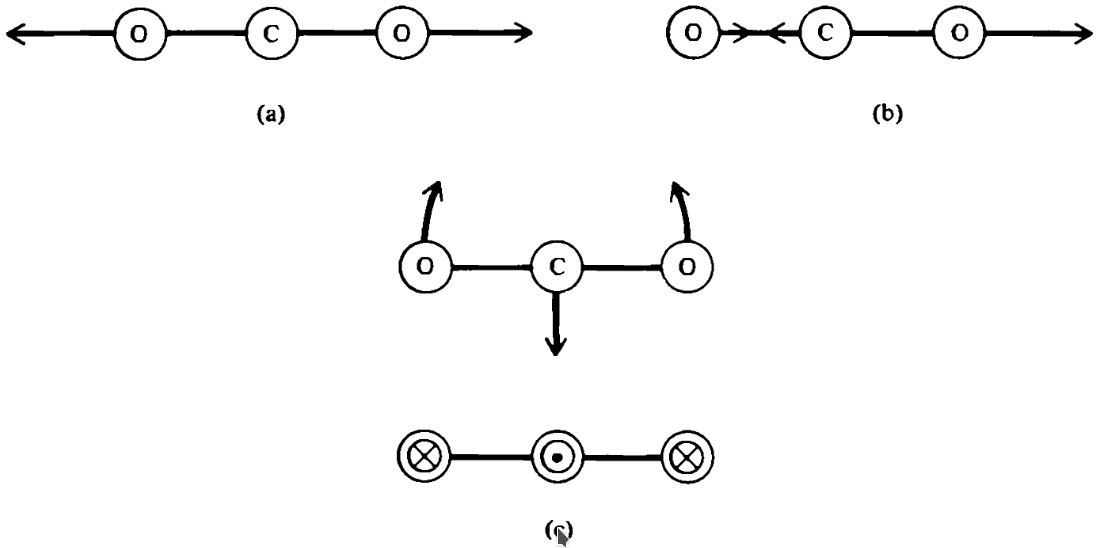
\includegraphics[width=0.8\linewidth]{co2.png}
	\caption{$CO_2$ normal coordinate analysis}%
	\label{fig:polyco2}
\end{figure}
With the normal coordinates then, the partition function is
\begin{equation*}
	q_{vib} = \prod_{j=1}^{\alpha}{\frac{e^{-\theta_{\nu_{j}/2T}}}{(1 -
	e^{-\theta_{\nu_{j}}/T}}}.
\end{equation*}
The energy and heat capacity are,
\begin{align*}
	E_{vib} &= Nk \sum_{j=1}^{\alpha}{\left(\frac{\theta_{\nu_j}}{2} +
			\frac{\theta_{\nu_j} e^{-\theta_{\nu_{j}/2T}}}{1 -
	e^{-\theta_{\nu_{j}}/T}}\right)}\\
		C_{v,vib} &= Nk
		\sum_{j=1}^{\alpha}{\left[\left( \frac{\theta_{\nu_{j}}}{T}\right)^2
			\frac{e^{-\theta_{\nu_{j}/2T}}}{1 - e^{-\theta_{\nu_{j}}/T}}.
	\right]}\\
\end{align*}

\section{Rotational Partition Function}%
\label{sec:polyrpf}
The rotational partition function depends a lot on the molecules inherent
symmetries. A theorem of rigid body motion which is the mode of energy in
consideration here, is always definable on 3 orthogonal principle axis where the
inertia tensor becomes diagonal. Each entry in the tensor is defined by
\begin{equation*}
	I_{ij} = \sum_{l=1}^{n}{m_l (x_{l,i} - x_{i,cm})(x_{l,j} - x_{j,cm})}.
\end{equation*}
So the theorem states there are orthogonal coordinate axes that make $I_{ij} =
0~\text{for}~i \ne j$.
\begin{equation*}
	\left[\begin{array}{c c c}
		I_{xx} & 0 & 0\\
		0 & I_{yy} & 0\\
		0 & 0 & I_{zz}
	\end{array}\right].
\end{equation*}
From the diagaonalization of the tensor $\overline{I}$ 4 cases exist: 3
identical $I$'s, 2 equal $I$'s, 3 unique $I$'s, and 2 identical nonzero $I$'s
and 1 zero $I$. These different cases are known as
spherical top, symmetric top, asymmetric top, and linear.

As a brief aside, a nomenclature for these 3 values have the subscripts as $I_a,
I_b, I_c$ and a convenient rescaling of the moments is given by,
\begin{equation*}
	{(\overline{A},\overline{B},\overline{C})} = \frac{h}{8\pi I_{a,b,c} c}.
\end{equation*}

\subsection{Linear Molecules}
For linear molecules, the problem is the same as the diatomic case. The moment
of inertia is given by $I = \sum_{i=1}^{n}{m_i r_i^2}$, where $r_{i}^2$ is the
distance from the center of mass. The final partition function is the same as
before
\begin{equation*}
	q_{rot} = \frac{8 \pi^2 IkT}{\sigma h^2} = \frac{T}{\sigma \Theta_r}.
\end{equation*}
Once again $\sigma$ is the symmetry number which represents the number of
indistinguishable configurations a molecule has.

\subsection{Non-Linear Molecules}
Non-linear rigid bodies have at least two different diagonal moments of
inertia. The principle axis are usually located on the axis of symmetry and
highly symmetric molecules usually have more of their moment of inertia
components the same.

\subsubsection{Spherical Tops}
The case of the spherical top applies to molecules like $CH_4$ and $CCl_4$ and
other highly symmetric molecules. The energy levels of this system are
\begin{align*}
	\varepsilon_j &= \frac{J(J+1)\hbar^2}{2I} \qquad J = 0,1,2,\ldots\\
	\text{with degeneracy}\\
	\omega_j &= (2J + 1)^2.
\end{align*}
The taking the classical approximation $q_{rot}$ is given by
\begin{equation*}
	q_{rot} = \frac{1}{\sigma}
	\int_{0}^{\infty}{(2J + 1)^2 e^{-J(J+1)\hbar^{2}/2kT}\d{J}}.
\end{equation*}
In addition, at large values of $J$ the $(J + 1) \approx J$, so
\begin{equation*}
	q_{rot} &= \frac{1}{\sigma}
	\int_{0}^{\infty}{4J^2 e^{-J^2 \hbar^{2}/2IkT}\d{J}}\\
\end{equation*}
Let,
\begin{align*}
	u &= 2J &\text{and} \quad
	\d{v} = 2J e^{-J^2 \hbar^{2}/2kT}\\
	\d{u} &= 2 \d{J}  &\text{and} \quad
	v = \frac{4IkT}{\hbar^2} e^{-J^2 \hbar^{2}/2IkT},
\end{align*}
Here, I note that the integral is directly analogous to that used to prove the
law of equipartition derived in Section\ref{sec:eoe}. Then, the final solution
is
\begin{equation*}
	q_{rot} = \frac{1}{\sigma}
	{\left( \frac{8\pi^{2/3} IkT}{h^2} \right)}^{3/2}.
\end{equation*}
Note that the $3/2$ power comes from the constant of $v$ and the
evaluation of $\int{v \d{u}}$ which provides 1 and $1/2$ power
respectively.

\subsubsection{Symmetric Tops}
The symmetric top also has a analytical quantum mechanical solution. A theorem
states that any rigid body with at least $n \ge 3$ fold axis of symmetry is at
least a symmetric top. The energy levels are
\begin{align*}
	\varepsilon_{JK} &= \frac{\hbar^2}{2}
	{\left( \frac{J(J+1)}{I_A} + K^2
	{\left[\frac{1}{I_c} - \frac{1}{I_{a}}\right]}
	\right)}\\
	J &= 0,1,2,\ldots
	~\text{and}~K = J, J-1, \ldots, -J\\
	\text{with degeneracy}\\
	\omega_{JK} &= (2J+1).
\end{align*}
$K$ represents the distribution of energy in the non symmetric axis. By
definition then,
\begin{equation*}
	q_{rot} = \frac{1}{\sigma}
	\sum_{J=0}^{\infty}{(2J+1) e^{-\alpha_A J(J+1)}}
	\sum_{K=-J}^{J}{e^{-(\alpha_C - \alpha_{A})K^2}},
\end{equation*}
with
\begin{equation*}
	\alpha_j = \frac{\hbar^2}{2I_j kT}.
\end{equation*}
The classical limit (integral) of this equation evaluates much the same as
previously using the results of the error function as has been repeatedly done,
\begin{equation*}
	q_{rot} = \frac{\pi^{1/2}}{\sigma}
	{\left(\frac{8\pi^2 I_A kT}{h^2}\right)}
	{\left(\frac{8\pi^2 I_C kT}{h^2}\right)}^{1/2}.
\end{equation*}
\subsubsection{Asymmetric Tops}
The case of asymmetric tops is only numerically solvable in quantum mechanics;
thus, a fully classical approach is necessary to get a closed form partition
function. The classical solution is of the same ilk as the other as one
might expect,
\begin{equation*}
	q_{rot} = \frac{\pi^{1/2}}{\sigma}
	{\left(\frac{8\pi^2 I_A kT}{h^2}\right)}^{1/2}
	{\left(\frac{8\pi^2 I_B kT}{h^2}\right)}^{1/2}
	{\left(\frac{8\pi^2 I_C kT}{h^2}\right)}^{1/2}.
\end{equation*}
With rotational temperatures,
\begin{equation*}
	q_{rot} = \frac{\pi^{1/2}}{\sigma}
	{\left(\frac{T^3}{\Theta_A \Theta_B \Theta_{C}}\right)}.
\end{equation*}

\subsubsection{Hindered Rotation}
If rotation around a particular bond --- such as the carbon-carbon bond in
ethane --- causes a meaningful change in potential the rotation is hindered.
Previously in this chapter, we have only considered molecules whose internal
rotation occurs in a equa-potential field or internal rotation is unhindered
(free). When internal rotation is free, such motion does not contribute to the
partition function. Taking the ethane example, such internal rotation must be
taken into consideration when deriving the partition function. Let's use the
potential energy of the rotation of the hydrogen in ethane as shown in
Figure~\ref{fig:polyhinderedrotation}.
\begin{figure}[htpb]
	\centering
	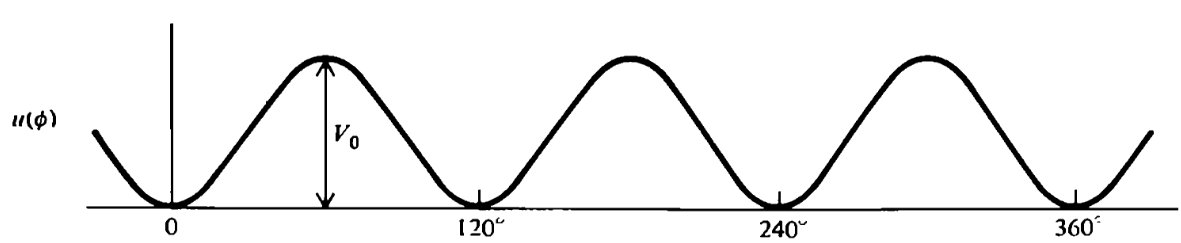
\includegraphics[width=0.8\linewidth]{hindered_rotation.png}
	\caption{Generic hindered rotation potential field}%
	\label{fig:polyhinderedrotation}
\end{figure}

At low temperatures where $kT \ll V_0$ the energy mode can be treated as a
harmonic oscillator around a energy minimum. If $kT \gg V_0$ the problem
rotation is free and a rigid rotor approximation is valid. However, when $kT
\approx V_0$ a different approach must be taken. In this case, we need an
analytical form of the potential, in this case $\frac{1}{2} V_0 (1 -
\cos{3\phi})$. The Schrödinger equation is difficult or impossible to solve
analytically, but the eigenvalues of the function are known.

\section{Thermodynamic Relations}%
\label{sec:polytr}
Here I copy some general thermodynamic relations,
\begin{align*}
	q &= q_{trans} q_{rot} q_{vib} q_{elec}\\
	  &= {\left(\frac{2\pi mkT}{h^3}\right)}^{3/2}V \cdot
		 \frac{\pi^{1/2}}{\sigma}
		 {\left(\frac{T^3}{\Theta_A \Theta_B \Theta_{C}}\right)}^{1/2}
		 {\left(\prod_{j=1}^{3n-6}{\frac{e^{-\theta_{\nu_{j}/2T}}}{(1 -
		 e^{-\theta_{\nu_{j}}/T})}}\right)}
		 \omega_{e1} e^{D_o /kT}\\
	\frac{-A}{NkT} &= \ln{\left(\frac{2\pi MkT}{h^2}\right)}
		 \frac{Ve}{N} + \ln{\left[\frac{\pi^{1/2}}{\sigma}
		 {\left(\frac{T^3}{\Theta_A \Theta_B \Theta_{C}}\right)}^{1/2}
		 \right]}
		 \sum_{j=1}^{3n-6}{\left(\frac{\Theta_{\nuj}}{2T} +
		 \ln{(1 - e^{-\Theta_{\nuj}/T})}\right)} +
		 \frac{D_e}{kT} + \ln{\omega_{e1}}\\
	\frac{E}{NkT} &= \frac{3}{2} + \frac{3}{2} +
		\sum_{j=1}^{3n-6}{\left(\frac{\Theta_{\nuj}}{2T} +
		\frac{\Theta_{\nuj}/T}{e^{\Theta_{\nuj}/T} - 1}\right)}-
		\frac{D_e}{kT}\\
	\frac{C_v}{Nk} &= \frac{3}{2} + \frac{3}{2} + 
		\sum_{j=1}^{3n-6}{\left({\left(\frac{\Theta_{\nuj}}{T}\right)} +
		\frac{e^{\Theta_{\nuj}/T}}{e^{\Theta_{\nuj}/T} - 1}\right)}\\
	\frac{S}{Nk} &= \ln{\left[\frac{2\pi MkT}{h^{2}}\right]}^{3/2}
	\frac{Ve^{5/2}}{N} + \ln{\left[\frac{\pi^{1/2} e^{3/2}}{\sigma}
	{\left(\frac{T^3}{\Theta_A \Theta_B \Theta_{C}}\right)}^{1/2}\right]}\\
	&+ \sum_{j=1}^{3n-6}{\left({\left(\frac{\Theta_{\nu_j}/T}%
	{e^{\Theta_{\nu_j}/T} - 1}\right)} - \ln{(1 -
	e^{-\Theta_{\nu_{j}/T}})}\right)} + \ln{\omega_{e1}}\\
	pV &= kNT.
\end{align*}
Notice that despite the more complicated molecular nature of polyatomic
molecules, the ideal gas law still ``pops'' out. This is because the ideal gas
law is a consequence of non interacting molecules or equivalently low density
systems not the features of the particles themselves. The other properties are
easily found from thermodynamic relationship that have been used previously.

Using these equations, entropy can be calculated more accurately than some
experiments. However, discrepancies can exist. For instance, carbon monoxide has
too weak a dipole moment to enforce the most energetically favorable arrangement
at low temperatures, so the molecules lack the kinetic energy to rearrange but
also are in a non-optimal arrangement. This kind of behavior is termed
\textit{residual} entropy.
